\subsection{CVSS TypeScript Implementation} \label{subsec:projektbericht-loesungsweg-typescript-cvss-online-calculator}

Dieses Kapitel geht auf die Details hinter der CVSS-Implementierung\footnote{\url{https://github.com/org-metaeffekt/metaeffekt-universal-cvss-calculator}} in TypeScript ein, wie sie im Universal CVSS Calculator\footnote{\url{https://www.metaeffekt.com/security/cvss/calculator}} der {\metaeffekt} verwendet wird.
In Abbildung \ref{fig:cvss-ts-calculator-class-diagram} kann das Klassendiagramm der TypeScript-Klassen mit allen Exports und Imports gefunden werden, welche in diesem Kapitel erklärt werden.

\begin{figure}[htbp] % here, top, bottom, separate page
    \centering
    \makebox[\textwidth][c]{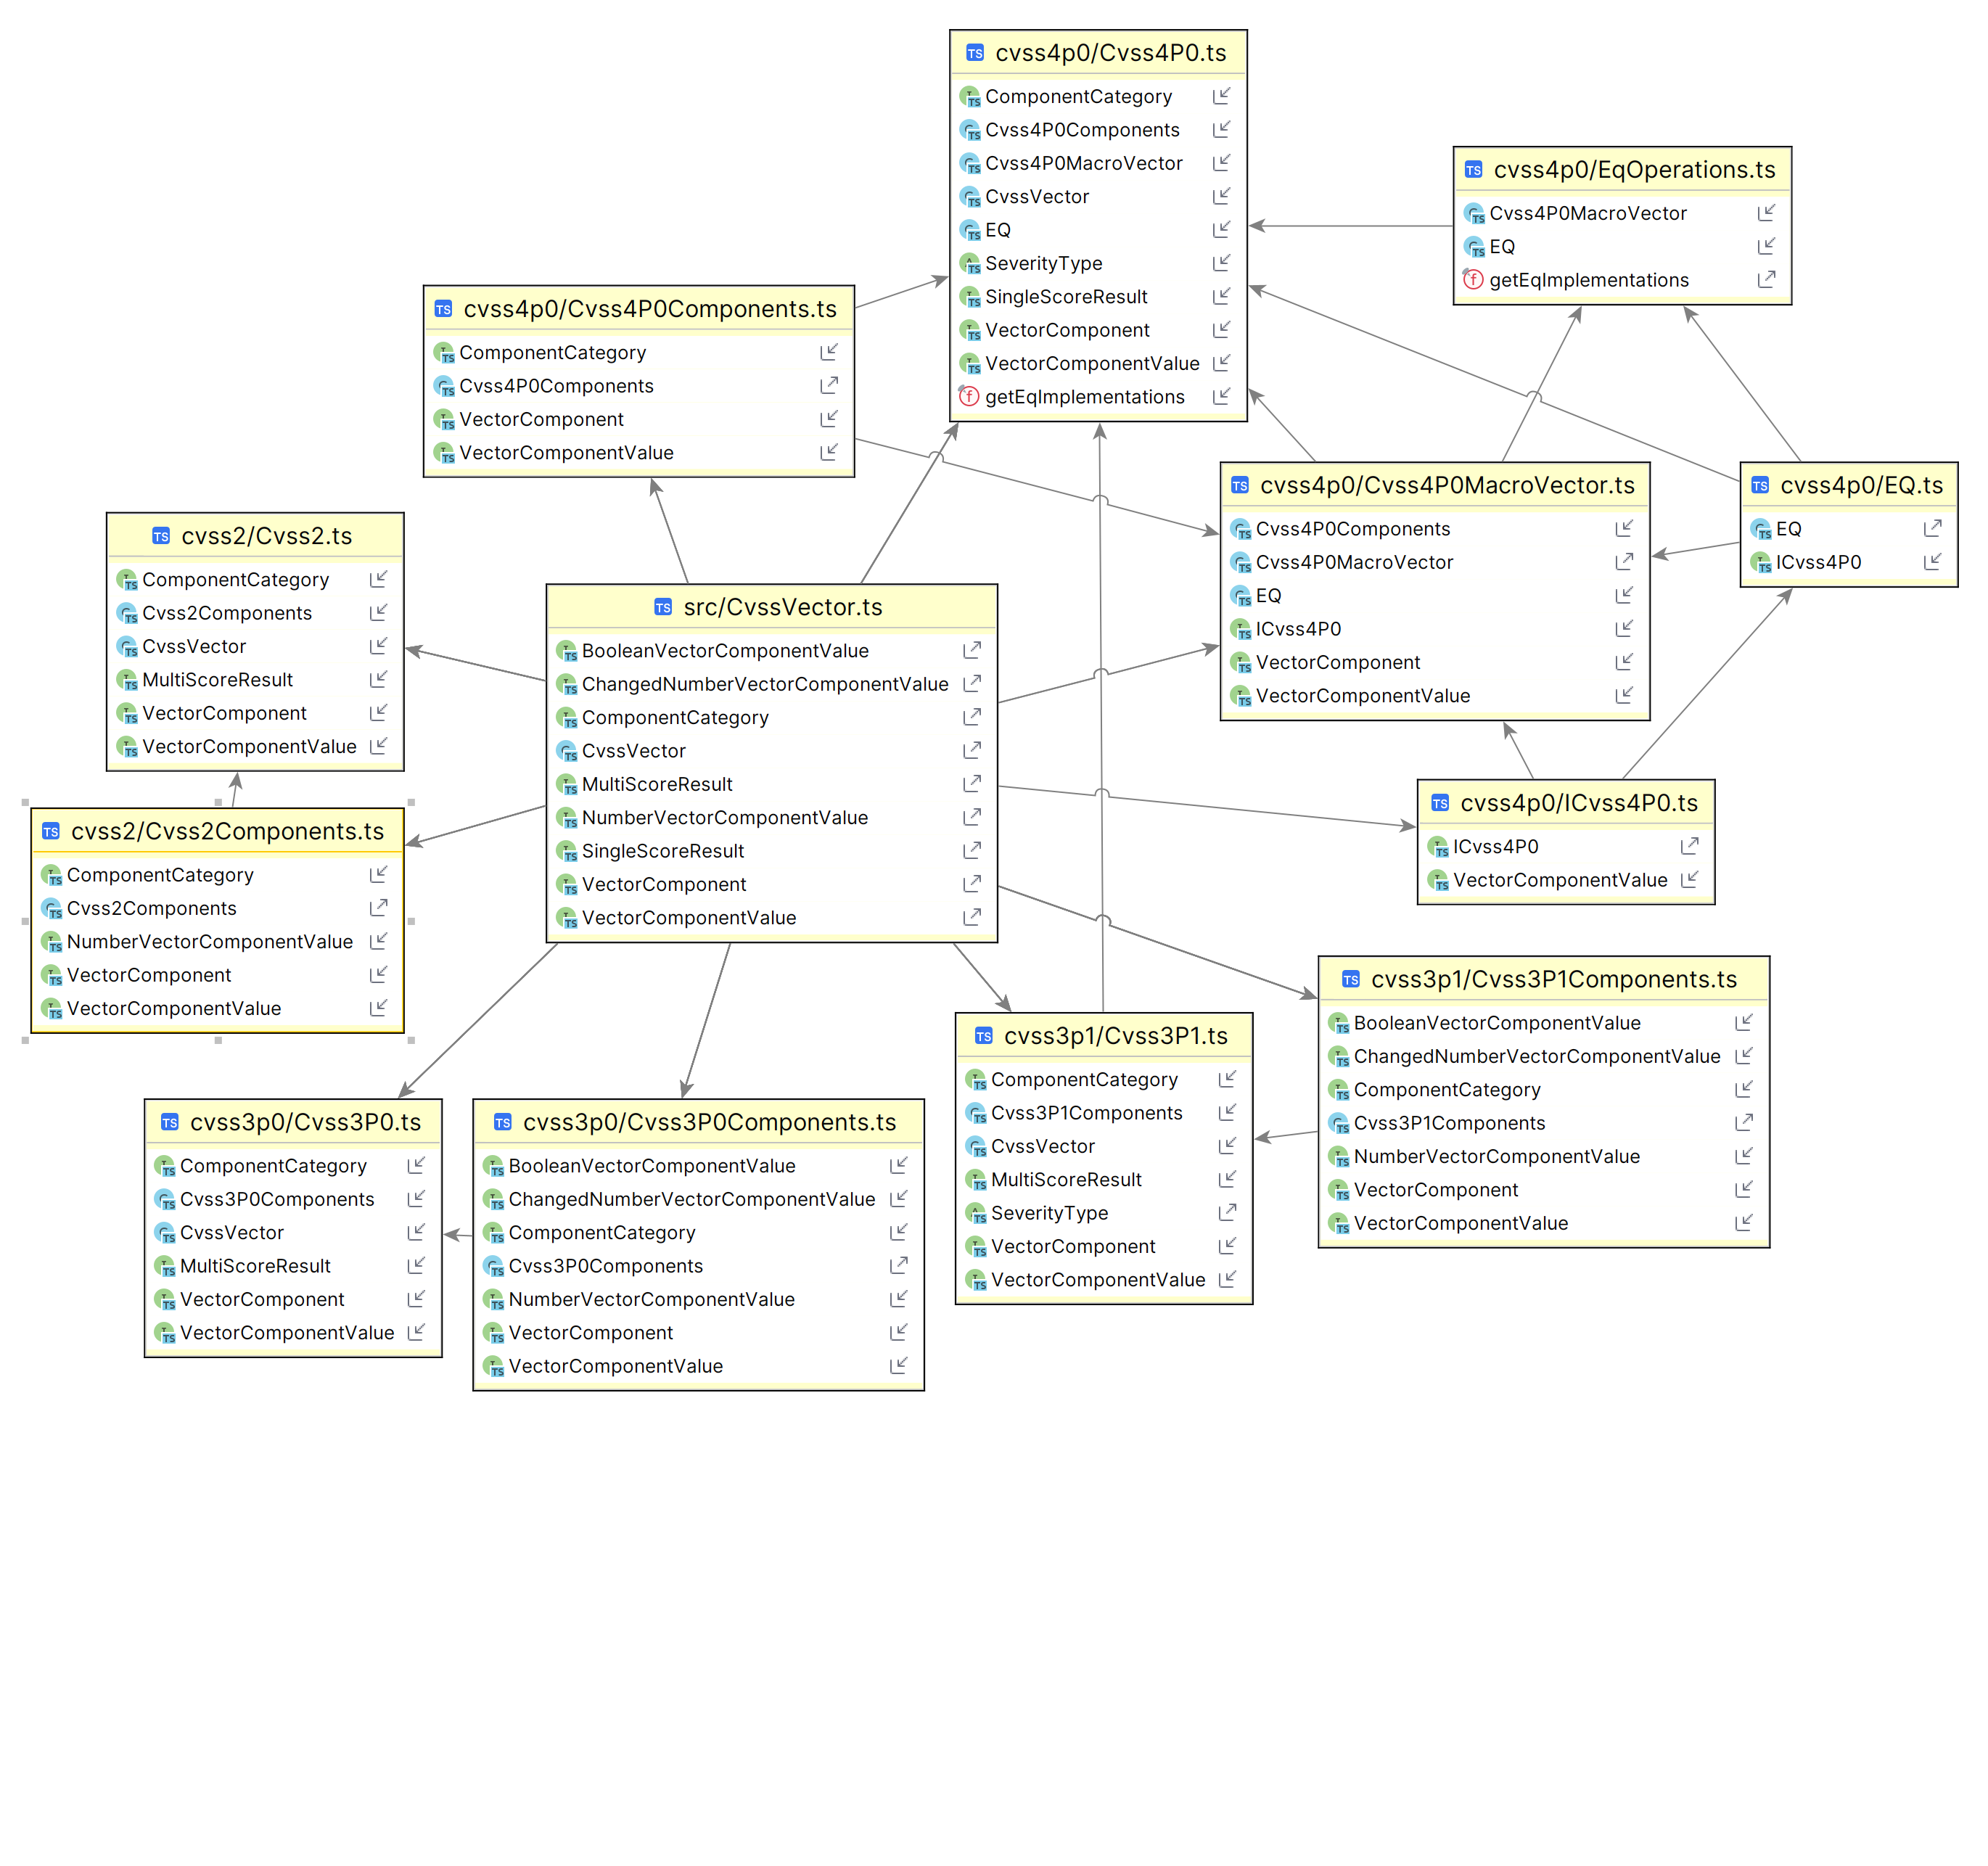
\includegraphics[width=1.2\textwidth, keepaspectratio]{res/grafiken/cvss-ts-calculator-class-diagram}}
    \caption{Klassendiagramm des CVSS-Rechners in TypeScript}
    \label{fig:cvss-ts-calculator-class-diagram}
\end{figure}

Da sich die Vektoren nur in ihren verwendeten Metriken, Metrikgruppen und der Score-Berechnung unterscheiden, kann recht viel der gemeinsamen Logik in eine Oberklasse \code{CvssVector} extrahiert werden.
In Listing \ref{lst:cvss-typescript-cvss-vector-class-attributes} wird ein Ausschnitt der recht schmalen Attributmenge und einigen relevanten Methoden gegeben.

\begin{lstlisting}[language=Java, label={lst:cvss-typescript-cvss-vector-class-attributes}, caption={CvssVector Klasse in TypeScript}]
export abstract class CvssVector<R extends BaseScoreResult> {
 components: Map<VectorComponent<VectorComponentValue>, VectorComponentValue>;

 public abstract calculateScores(normalize: boolean): R;
 public abstract getVectorName(): string;
 public applyComponent(setComponent: VectorComponent<VectorComponentValue>, setValue: VectorComponentValue) { ... }
 public getComponent<T extends VectorComponentValue>(component: VectorComponent<T>): T { ... }
}
\end{lstlisting}

Generell ist das Schema jeder Berechnungsfunktion mit \code{calculateScores} gleich, denn es wird immer ein Objekt mit mindestens einem Overall-Score und je nach Vektorversion zusätzliche Scores konstruiert und zurückgegeben.
In Listing \ref{lst:cvss-typescript-cvss-3P1-calculateScores} wird dies anhand von CVSS 3.1 gezeigt, da diese Version einige Besonderheiten darstellt.
CVSS 3.1 hat unter anderem das Problem, dass der sog. \qt{Environmental} und \qt{Temporal} Score nicht auf eine Spanne von 0-10 normalisiert werden, sondern nur bis 6.0 oder 3.9 reichen.
Mit einem \code{normalize}-Parameter können diese scores auf die Spanne von 0-10 gemappt werden.
Zudem kann nicht immer jeder Score berechnet werden, denn zu den Scores müssen immer mindestens die entsprechenden Metriken vorhanden sein.

\begin{lstlisting}[language=Java, label={lst:cvss-typescript-cvss-3P1-calculateScores}, caption={CVSS 3.1 Score-Berechnung in TypeScript}]
calculateScores(normalize: boolean = false): MultiScoreResult {
    const base = isBaseFullyDefined();
    const temp = isAnyTemporalDefined();
    const env = isAnyEnvironmentalDefined();
    return {
        base: base ? round(baseScore(), 1) : undefined,
        impact: base ? normalize(round(impactScore(), 1), normalize ? 6.0 : 10) : undefined,
        exploitability: base ? normalize(round(exploitabilityScore(), 1), normalize ? 3.9 : 10) : undefined,
        temporal: base && temp ? round(temporalScore(), 1) : undefined,
        environmental: base && env ? round(environmentalScore(), 1) : undefined,
        modifiedImpact: base && env ? normalize(round(Math.max(0, adjustedImpactScore()), 1), normalize ? 6.1 : 10) : undefined,
        overall: round(overallScore(), 1),
        vector: toString()
    };
}
\end{lstlisting}

Die einzelnen Score-Berechnungsmethoden wurden von der Spezifikation\footnote{\url{https://www.first.org/cvss/v3.1/specification-document\#CVSS-v3-1-Equations}} übernommen und ähneln sich alle stark.
Ein typisches Beispiel ist die Berechnung des Impact-Scores, bei der auf diverse Metriken (unterschiedlichen Datentyps) zugegriffen wird und diese mit weiteren konstanten Werten verrechnet werden.
In Listing \ref{lst:cvss-typescript-cvss-3P1-calculateExactImpactScore} ist der dazugehörige Code zu finden.
\begin{align*}
    \text{ISS} &= 1 - [ (1 - \text{Confidentiality}) \times (1 - \text{Integrity}) \times (1 - \text{Availability}) ] \\
    \text{If Scope is Unchanged:} & \quad 6.42 \times \text{ISS} \\
    \text{If Scope is Changed:} & \quad 7.52 \times (\text{ISS} - 0.029) - 3.25 \times (\text{ISS} - 0.02)^{15}
\end{align*}

\begin{lstlisting}[language=Java, label={lst:cvss-typescript-cvss-3P1-calculateExactImpactScore}, caption={CVSS 3.1 Impact Score-Berechnung in TypeScript}]
public calculateExactImpactScore(): number {
 const iss = 1 - ((1 - getComponent(C).value) * (1 - getComponent(I).value) * (1 - getComponent(A).value));

 if (getComponent(S).value) return SCOPE_CHANGED_FACTOR * (iss - 0.029) - 3.25 * Math.pow(iss - 0.02, 15);
 else return SCOPE_UNCHANGED_FACTOR * iss;
}
\end{lstlisting}

\subsubsection{CVSS:4.0 TypeScript Implementierung} \label{subsec:projektbericht-loesungsweg-typescript-cvss-online-calculator-cvss-4P0}

Etwas anders verhält es sich mit der Version 4.0 von CVSS, welche nur einen einzigen Score berechnet und dazu keine statischen Formeln, sondern höhere mathematische Konzepte verwendet.
Laut der Dokumentation und Entwicklungsgeschichte von CVSS 4.0 \cite{CVSSv4.0Specification} wurden die 15 Millionen möglichen CVSS-Vektoren automatisiert in 270 Äquivalenzgruppen aufgeteilt und einer Expertengruppe mit 50 Teilnehmern bereitgestellt, die diese absolut dem Schweregrad entsprechend einordnen sollten.
Dadurch konnte eine durchschnittliche Liste an Vektoren mit aufsteigenden Schweregraden berechnet werden, welcher recht einfach linear die CVSS-Scores von 0 bis 10 statisch vergeben und in einer Lookup-Tabelle der Öffentlichkeit zur Verfügung gestellt wurde.

Bei der Berechnung der Scores wird nun der initiale Input-Vektor mit seinen 32 Metriken auf nur 6 Dimensionen über diverse Regeln auf einen sog. \qt{MakroVektor} reduziert, um durch eben diese Lookup-Tabelle einen entsprechenden Basis-Score zu erhalten.
Nun wären allerdings 270 Scores etwas wenig, um die Vielfalt und den Detailgrad aller 15 Millionen Kombinationen darzustellen.
Daher wird ein Interpolationschritt dahinter geschaltet, der den Großteil der Berechnungslogik einnimmt.

Die folgenden Formeln werden nicht im Standard aufgeführt, da dieser sich eher mit den Konzepten hinter der Berechnung beschäftigt und nicht mit den eigentlichen Berechnungsmethoden.
Die Formeln und Teile der Bezeichner wurden aus der Implementierung abgeleitet und die Konzepte entsprechend angepasst.

\begin{align*}
    \text{ScoreInterpolated}(V) &= \text{ScoreBase}(MV) - \text{Mean}(\text{ScoreEQ}) \\
    \text{ScoreEQ} &= \text{ProportionDistance}(V, EQ) \times \text{ScoreRange}(MV, EQ) \\
    \text{ProportionDistance}(V, EQ) &= \frac{\text{SeverityDistance}(V, \text{MacroVector})}{\text{Depth}(\text{MacroVector})}
\end{align*}

Um die Formeln zu verstehen, muss verstanden werden, dass es zwei unterschiedliche Skalen mit verschiedenen Bedeutungen gibt:

\begin{description}
    \item[Severity Distance Scale] Diese Skala ist mit den Vektormetriken und deren möglichen Werten verbunden.
    Eine Änderung von $\pm 1$ auf dieser Skala stellt eine Änderung eines einzelnen Metrikwerts um einen Wert nach oben oder unten dar (ernster, weniger ernst).
    \item[CVSS Score Scale] Sie quantifiziert die Schwere der Schwachstelle in einem Bereich von 0 bis 10, wobei höhere Werte auf schwerwiegendere Schwachstellen hinweisen.
    Die kleinste mögliche Änderung auf dieser Skala ist $0.1$.
\end{description}

Damit können die folgenden Werte und Formeln definiert werden:

\begin{itemize}[noitemsep]
    \item \textbf{MV} ist der aus dem ursprünglichen Vektor berechnete MakroVektor.
    \item \textbf{EQ} ist eine sog.\ Äquivalenzgruppe, die aus einer Menge an Definitionen für Kriterien, wann ein Vektor innerhalb dieser Gruppe ist und eine Liste der Vektoren mit den höchstmöglichen Scores die in dieser Gruppe sind, führt.
    \item \textbf{ScoreInterpolated$(V)$} ist der endgültig berechnete Score für den Vektor.
    \item \textbf{ScoreBase$(MV)$} ist der Score für den MacroVector, bestimmt durch Nachschlagen in der Tabelle.
    \item \textbf{Mean$(scores)$} berechnet den Durchschnittsscore über alle EQ (Äquivalenz)-Gruppen, die für den Vektor zutreffen.
    \item \textbf{ScoreEQ} ist eine Liste von proportionalen Score-Anpassungen für jede EQ-Gruppe, berechnet durch eine Unterformel.
    \item \textbf{ProportionDistance$(V, EQ)$} (severity distance scale) berechnet als die Severity Distance geteilt durch die Tiefe des MacroVectors für diese EQ-Gruppe, ergibt einen Wert zwischen 0 und 1.
    \item \textbf{SeverityDistance$(V, MacroVector)$} (severity distance scale) ist die Anzahl der Metrikwertänderungen, die benötigt werden, um den Vektor $V$ vom Vektor mit der höchsten Schwere innerhalb desselben MacroVectors zu erreichen.
    \item \textbf{Depth$(MacroVector)$} (severity distance scale) ist die Gesamtanzahl der Metrikwertänderungen innerhalb eines MacroVectors von seinem höchsten bis zu seinem niedrigsten Schwerevektor.
    Diese ist je nach MakroVektor unterschiedlich, da jeder unterschiedlich breit sein kann.
    \item \textbf{ScoreRange$(MV, EQ)$} (CVSS score scale) ist der Unterschied im Score zwischen dem höchsten und niedrigsten Schwerevektor innerhalb des MacroVectors für eine gegebene EQ-Gruppe.
    Sie repräsentiert die effektive Score-Spanne innerhalb eines MakroVektors.
\end{itemize}

In Listing \ref{lst:cvss-typescript-cvss-4P0-calculateOverallScore-pseudocode} wird der Pseudocode für die Berechnung des Scores gezeigt, wie er sonst in der Cvss4P0-Klasse gefunden werden kann.

\begin{lstlisting}[language=Java, label={lst:cvss-typescript-cvss-4P0-calculateOverallScore-pseudocode}, caption={CVSS 4.0 Score-Berechnung Pseudocode}]
function calculateOverallScore(inputVector):
  if not isBaseFullyDefined(inputVector):
      return 0.0

  if isNoImpactOnSystem(inputVector):
      return 0.0

  // implementations for handling different equivalence groups
  eqOperations = getEqImplementations()

  macroVector = getMacroVector(inputVector)
  performSafetyCheck(macroVector)
  macroVectorScore = lookupTableScore(macroVector)

  allHighestSeverityVectors = []
  for eqOp in eqOperations:
    allHighestSeverityVectors.add(eq.getHighestSeverityVectors(macroVector))

  highestSeverityVectorCombinations = generateCvssPermutations(allHighestSeverityVectors)
  if highestSeverityVectorCombinations is empty:
      return 0.0 // no max vectors found
  highestSeveritySeverityDistances = calculateSeverityDistances(highestSeverityVectorCombinations)

  meanScoreAdjustment = new AverageCalculator()
  for eqOp in eqOperations:
      nextLessSevereMacroVector = eqOp.deriveNextLowerMacro(macroVector)
      nextLowerMacroScore = eqOp.lookupScoresForNextLowerMacro(nextLessSevereMacroVector)
      availableSeverityReduction = macroVectorScore - nextLowerMacroScore

      macroVectorDepth = lookupMacroVectorDepth(eqOp, macroVector)
      severityDistanceFromThisToHighestSeverity = eqOp.sumSeverityDistances(highestSeveritySeverityDistances)

      if not isNaN(availableSeverityReduction) and macroVectorDepth != 0.0:
          percentageToNextSeverityDistance = severityDistanceFromThisToHighestSeverity / macroVectorDepth
          normalizedSeverityDistance = percentageToNextSeverityDistance * availableSeverityReduction
          meanScoreAdjustment.add(normalizedSeverityDistance)

  adjustedOriginalMacroVectorScore = macroVectorScore - meanScoreAdjustment.average()

  return adjustScoreWithinValidRange(adjustedOriginalMacroVectorScore)
\end{lstlisting}
